\documentclass[compress,xcolor=table]{beamer}

% Packages
\usepackage[american]{babel}
\usepackage[utf8]{inputenc}
\usepackage[T1]{fontenc}
\usepackage{datetime}
\usepackage{graphicx}
\usepackage{subcaption}
\usepackage{csquotes}


\graphicspath{{images/}}



% Possible options of the package (add/remove below in \usetheme call):
%  - nosectionpages: no pages between sections
%  - flama: use flama font, requires xelatex/lualatex + the font to compile
%  - compressminiframes: put the heading list bullets indications pages on 1 line
\usetheme[compressminiframes]{Davis}

% Title page
\title{Yazılım Mühendisliği \newline Özel Konular  }
\foottitle{QMOOD Modeli İle Nesneye Dayalı Yazılım Kalitesi Ölçümü} % optional, printed at the bottom of the slides, by default same as title, can be useful to rewrite when title has a newline for example
\subtitle{QMOOD Modeli İle Nesneye Dayalı Yazılım Kalitesi Ölçümü} % optional subtitle
\date{\formatdate{12}{01}{2021}}
\author{Serdar ATEŞ             \& Furkan TOPTAŞ     \&  Bilal BAŞULAŞ}
\institute{162805009               \& 162805008                \& 162805005} % Optional

% Biblatex
\usepackage[backend=biber, style=apa]{biblatex}
\bibliography{library.bib}
\renewcommand*{\bibfont}{\footnotesize}


%%%%
%% BEGIN OF SLIDES
%%%%

\begin{document}

\begin{frame}[plain]
\titlepage
\setcounter{framenumber}{0}
\end{frame}

\section{İçindekiler} \subsection{}

\begin{frame}{İçindekiler}

\begin{block}{1- Giriş}
		
\begin{itemize}
\item İncelenen Proje Hakkında Bilgilendirme
\item Kullanılan Araçlar
\end{itemize}
		
\end{block}
	
    \begin{block}{2- Kullanılan Yaklaşımlar}
		
\begin{itemize}
\item İncelenen Proje Hakkında Bilgilendirme
\item Kullanılan Araçlar
\end{itemize}
		
\end{block}
  \begin{block}{3-Değerlendirme}
		

		
\end{block}
  \begin{block}{4- Sonuç}
	

		
\end{block}

\end{frame}



\section{Giriş} \subsection{}

\begin{frame}{İncelenen Proje Hakkında Bilgilendirme}
\begin{block}{İncelenen Proje Hakkında Bilgilendirme}
		
\begin{itemize}
\item Android Studio Platformu
\item Android Studio ve Android SDK
\item Java Programlama Dili
\item Nesneye Dayalı Programlama Prensipleri
\item Son 2 Yıllık Süreç Değişikleri
\end{itemize}
		
\end{block}


\end{frame}
\begin{frame}{Kullanılan Araçlar}
\begin{block}{Kullanılan Araçlar}
		
\begin{itemize}
\item Metric Reloded
\item Source Monitor
\end{itemize}
		
\end{block}


\end{frame}

\begin{frame}{Kullanılan Araçlar: Metric Reloaded}
\begin{figure}
\vspace{-.8cm}
   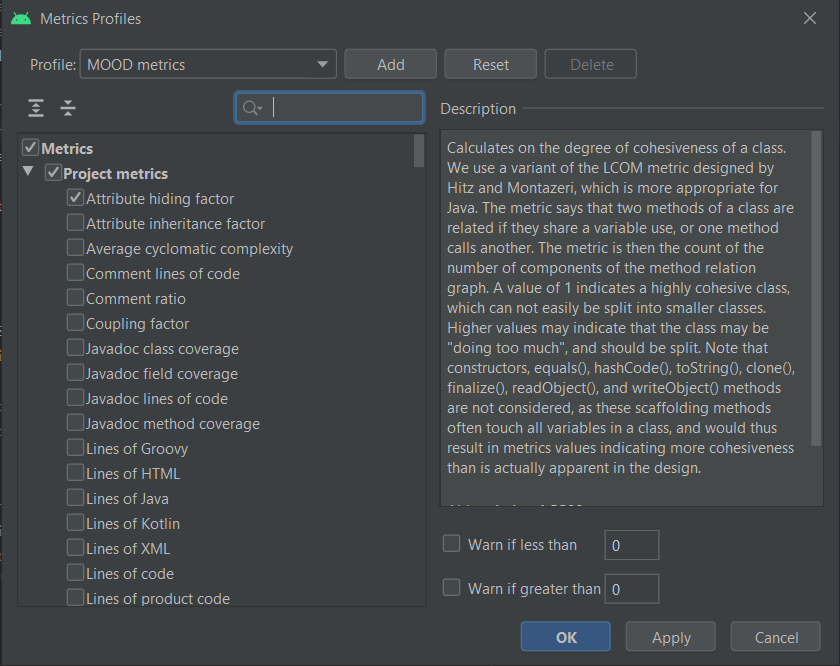
\includegraphics[width = \textwidth, height = 7.4 cm]{QMOODimage/android-metrik-1.png}
\end{figure}
\end{frame}
\begin{frame}{Kullanılan Araçlar: Metric Reloaded}
\begin{figure}
\vspace{-.8cm}
   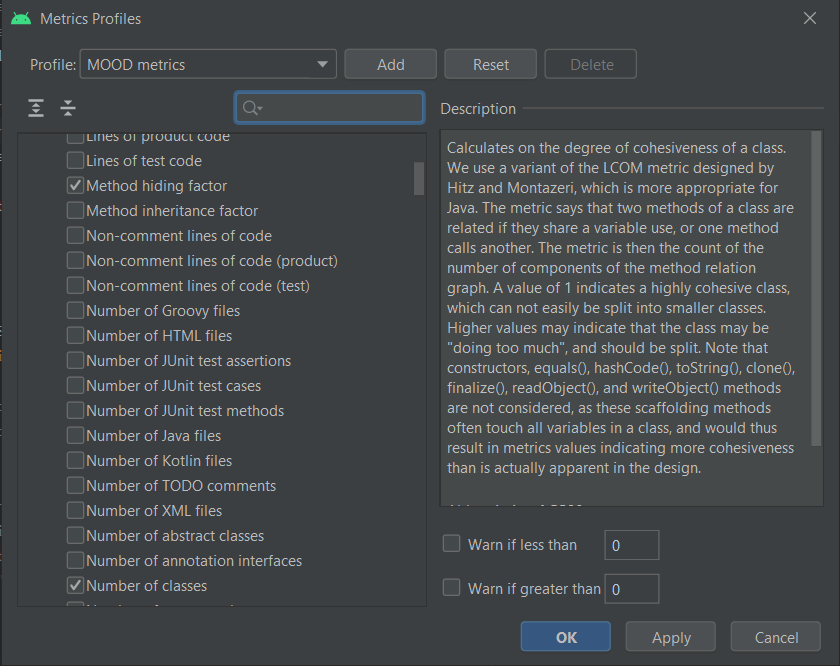
\includegraphics[width = \textwidth, height = 7.4 cm]{QMOODimage/android-metrik-2.png}
\end{figure}
\end{frame}

\begin{frame}{Kullanılan Araçlar: Metric Reloaded}
\begin{figure}
\vspace{-.8cm}
   \includegraphics[width = \textwidth, height = 7.4 cm]{QMOODimage/android-metrik-3.png}
\end{figure}
\end{frame}
        
        \begin{frame}{Kullanılan Araçlar: Metric Reloaded}
\begin{figure}
\vspace{-.8cm}
   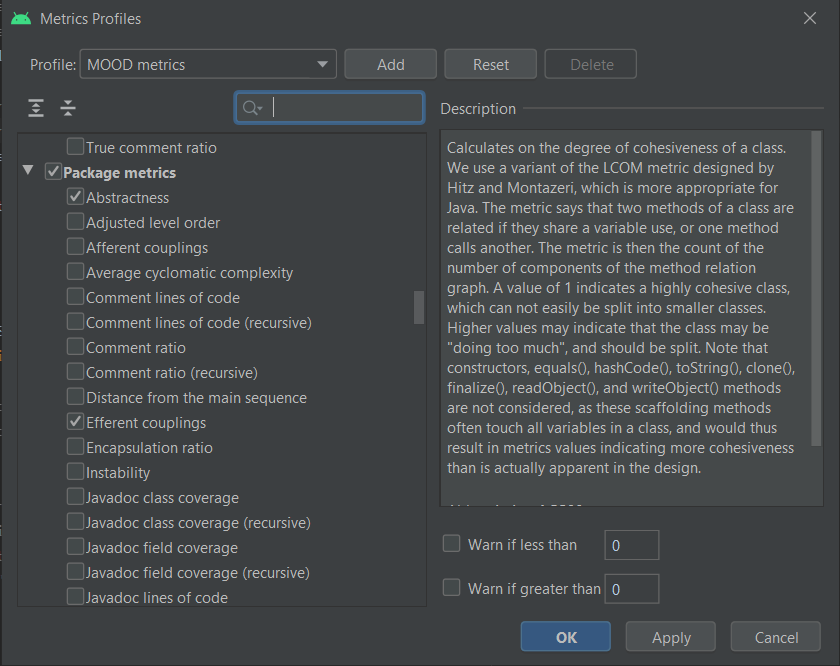
\includegraphics[width = \textwidth, height = 7.4 cm]{QMOODimage/android-metrik-4.png}
\end{figure}
\end{frame}
        
        \begin{frame}{Kullanılan Araçlar: Metric Reloaded}
\begin{figure}
\vspace{-.8cm}
   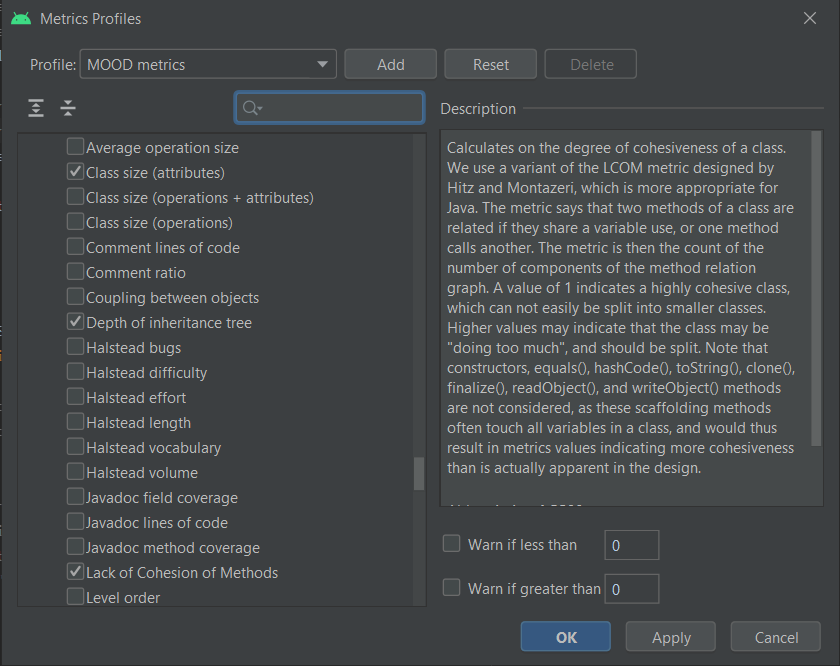
\includegraphics[width = \textwidth, height = 7.4 cm]{QMOODimage/android-metrik-5.png}
\end{figure}
\end{frame}
        
        \begin{frame}{Kullanılan Araçlar: Metric Reloaded}
\begin{figure}
\vspace{-.8cm}
   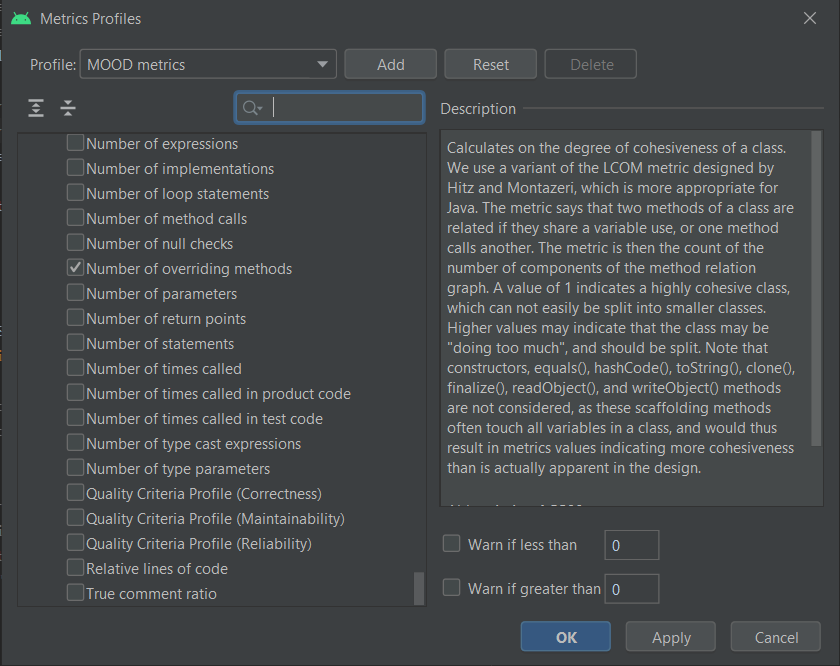
\includegraphics[width = \textwidth, height = 7.4 cm]{QMOODimage/android-metrik-6.png}
\end{figure}
\end{frame}
        
        \begin{frame}{Kullanılan Araçlar: Source Monitor}

\begin{figure}
\vspace{-.8cm}
   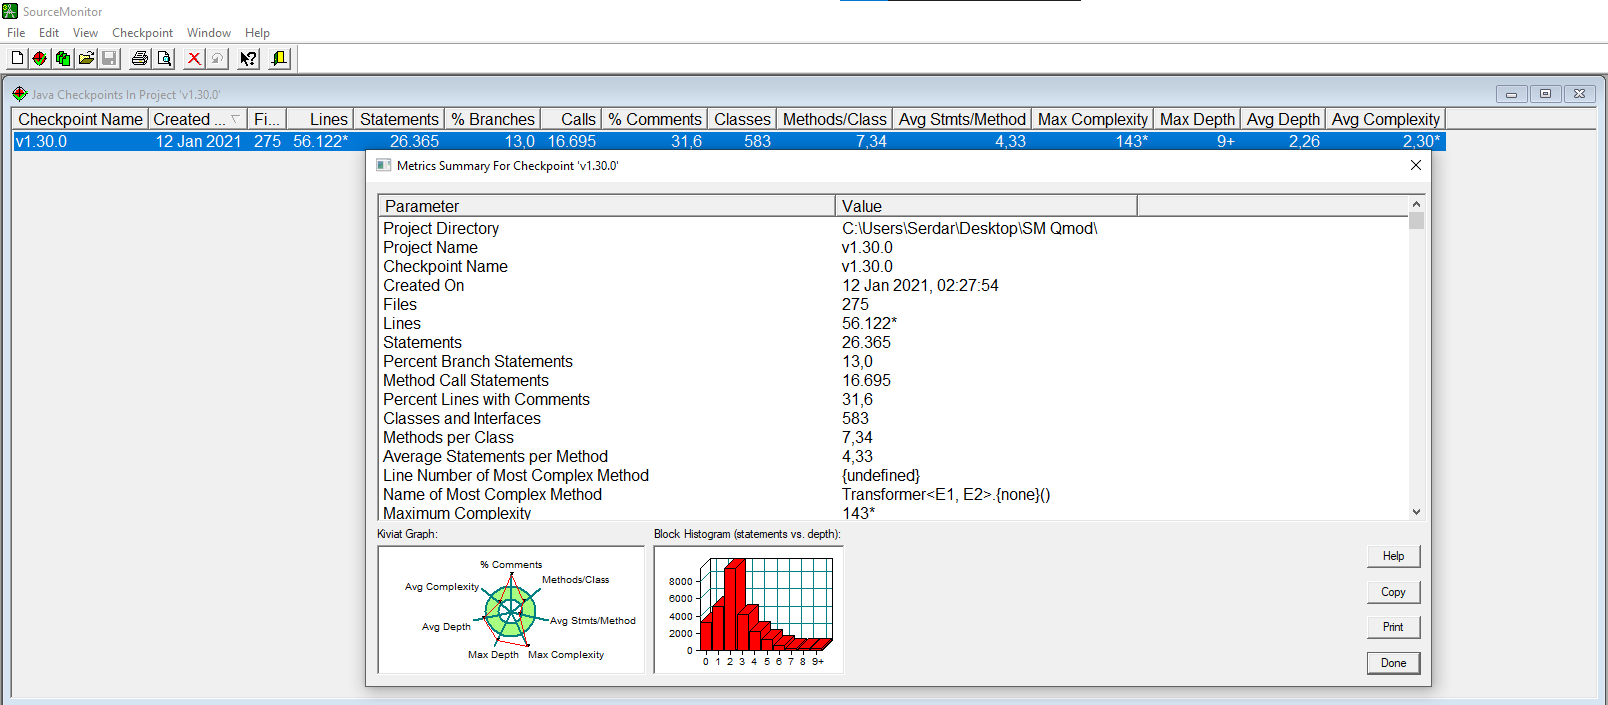
\includegraphics[width = \textwidth, height = 6.0 cm]{QMOODimage/grafik 2.png}
\end{figure}

\end{frame}
        \section{Kullanılan Yaklaşımlar} \subsection{}
        \begin{frame}{QMOOD Modeli}
\begin{block}{}
		
\begin{itemize}
\item Hiyerşik (Katmanlı) Yapı
\item (L1) Tasarım Kalitesi Nitelikleri
\item (L2) Tasarım Kalitesi Özellikleri
\item (L3) Tasarım Kalitesi Metrikleri
\item (L4) Tasarım Kalitesi Bileşenleri
\item (L3) Tasarım Kalitesi Bileşenlerinin Ölçülmesi
\end{itemize}
		
\end{block}
\end{frame}

\begin{frame}{QMOOD Modeli}
\begin{block}{(L3) Tasarım Kalitesi Metrikleri}
		
\begin{itemize}
\item (DSC) Design Size in Classes
\item (NOH) Number of Hierarchies
\item (ANA) Average Number of Ancestors
\item  (DAM) Data Access Metric
\item  (DCC) Direct Class Coupling
\item (CAM) Cohesion Among Methods in Class
\item  (MOA) Measure of Aggregation
\item  (MFA) Measure of Function Abstraction
\item (NOP) Number of Polymorphic Methods
\item  (CIS) Class Interface Size
\item  (NOM) Number of Methods



\end{itemize}

		
\end{block}
\end{frame}

\begin{frame}{QMOOD Modeli}
\begin{block}{(L4) Tasarım Kalitesi Bileşenleri}
		
\begin{itemize}
\item of Classes => (DSC)
\item Avg. Depth of Inheritance Hierarchy => (NOH)
\item Depth of Inheritance Tree =>(ANA)
\item X ( of Private + of Protected)/(of Total Fields) => (DAM)
\item of Coupling => (DCC)
\item 1-LCOM => (CAM)
\item of Data Declarations for User Def. Classes=> (MOA)
\item of Overridden Meth. / of Total Meth. =>  (MFA)
\item of Interfaces =>  (NOP)
\item of Public Methods =>  (CIS)
\item Total of Methods =>  (NOM)






\end{itemize}

		
\end{block}
\end{frame}


\begin{frame}{Hesaplanan Tasarımın Metrikleri}
\begin{block}{Metric Reloded ile}
		
\begin{itemize}
\item DAM
\item DCC
\item MOA
\item CIS
\item NOM
\item DSC
\item ANA
\item CAM
\item MFA
\item NOP






\end{itemize}

		
\end{block}


\begin{block}{Source Monitor ile}
	
\begin{itemize}
\item NOH






\end{itemize}

		
\end{block}


\end{frame}

        
        
        
        
        
        
        \begin{frame}{Hesaplanan Tasarımın Metrikleri}
\begin{block}{ }
		
\begin{itemize}
\item Metriklerin Uygun Şekilde Aynı Düzeye Çekilmesi
\item En Yüksek Puana Göre Normalizasyon
\item Tasarım Özelliklerine Geçiş(L3 =>L2)
\item Tasarım Niteliklerine Geçiş(L2 =>L1)
\item Hesaplanan Tasarımın Nitelikleri için normalizasyon



\end{itemize}

		
\end{block}
\end{frame}
        

        
\section{Değerlendirme} \subsection{}



\begin{frame}{Kalite Nitelikleri Grafiği}
\begin{figure}

\vspace{-.8cm}
   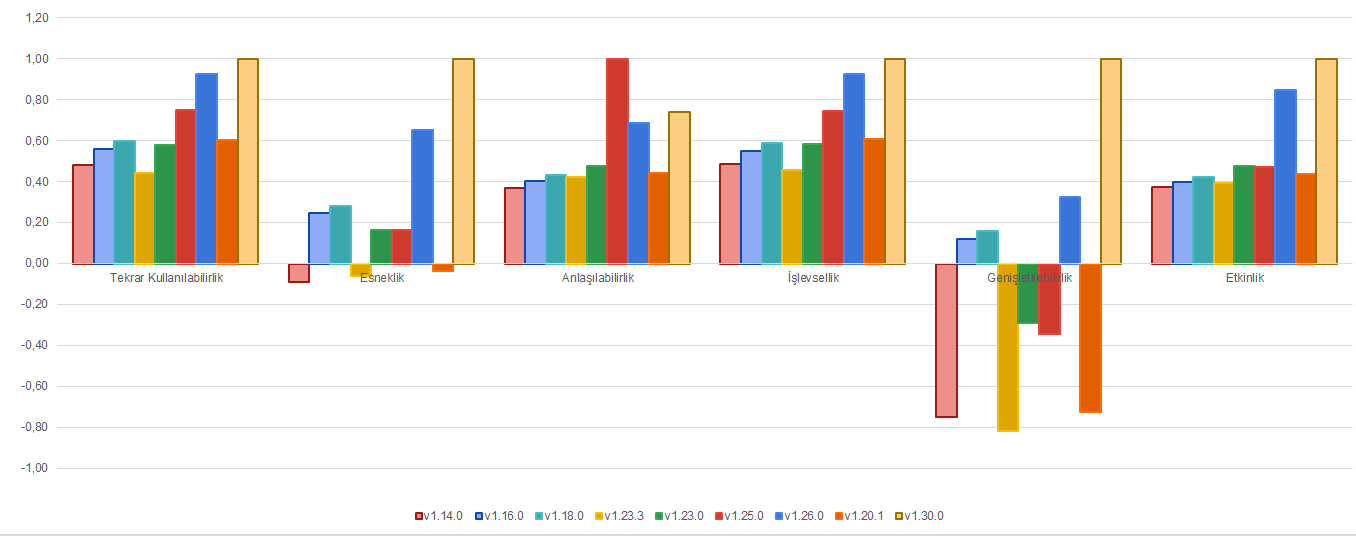
\includegraphics[width = \textwidth, height =6cm]{QMOODimage/grafik 1.png}
\end{figure}
\vspace{-1cm}
\begin{itemize}
   
\end{itemize}
\end{frame}


\section{Sonuç} \subsection{}
 \begin{frame}{Sonuç}
 
 Belirlenen nitelikler baz alındığında bu yazılım ürünün bazı güncellemelerinde kalite analamında iyileştirilme yapılmasına rağmen bazı güncellemelerde ise bu kalite nitelikleri düşmüştür.
 
 
\begin{block}{Genel Sürüm Güncellemelerinde Kalite Niteliği Değişimi }
		
\begin{itemize}
\item v14.0 => Stabil
\item v16.0 => Olumlu
\item v18.0 => Stabil
\item v20.1 => Olumsuz
\item v23.0 => Olumsuz
\item v23.3 => Olumlu
\item v25.0 => Olumlu
\item v26.0 => Olumsuz
\item v30.0 => Stabil



\end{itemize}

		
\end{block}
\end{frame}

 \begin{frame}{Sonuç}
\begin{block}{Hedeflnen Performansa Yakın Çünkü; }
		
\begin{itemize}
\item Güncellemeler Sık Aralıklarla Yapıldığından Sonuç Beklenelinen Gibi Olmamıştır.
\item Frameworkleri Sürekli Refactoring Etme Süreci
\item Güncellemelerde Çok Büyük Eklemeler Ve Çıkarılmalar Yapıldığından Kalite Nitelikleri Arasında Tam Doğrusal Bir Bağıntı Oluşmamıştır
\item Gradle Güncellemeleri Projeyi Her Versiyonda Zorlamıştır.
\item Android Studio Versiyon Güncelleme Süreci 
\item Android SDK Güncellemelerini Her Versiyonda Projeye Adaptasyon Süreci
\item QMOOD ile Mobil Uygulamnın modellemesi başarılı



\end{itemize}

		
\end{block}
\end{frame}






\section{Hazırlayanlar} \subsection{}
\begin{frame}


\begin{block}{ }
		
\begin{itemize}
\item Serdar ATEŞ - 162805009
\item Furkan TOPTAŞ - 162805008
\item Bilal BAŞULAŞ - 162805005



\end{itemize}

		
\end{block}
\end{frame}




\end{document}

